% !TeX spellcheck = en_US
\documentclass[french]{yLectureNote}

\title{Mécanique}
\subtitle{Mécanique du point}
\author{Paulhenry Saux}
\date{\today}
\yLanguage{Français}

\professor{S.Deheuvels}%sebastien.deveuhels.irap.omp.eu

\usepackage{graphicx}%----pour mettre des images
\usepackage[utf8]{inputenc}%---encodage
\usepackage{geometry}%---pour modifier les tailles et mettre a4paper
%\usepackage{awesomebox}%---pour les boites d'exercices, de pbq et de croquis ---d\'esactiv\'e pour les TP de PC
\usepackage{tikz}%---pour deiffner + d\'ependance de chemfig
\usepackage{tkz-tab}
\usepackage{chemfig}%---pour deiffner formules chimiques
\usepackage{chemformula}%---pour les formules chimiques en \'equation : \ch{...}
\usepackage{tabularx}%---pour dimensionner automatiquement les tableaux avec variable X
\usepackage{awesomebox}%---Pour les boites info, danger et autres
\usepackage{menukeys}%---Pour deiffner les touches de Calculatrice
\usepackage{fancyhdr}%---pour les en-t\^ete personnalis\'ees
\usepackage{blindtext}%---pour les liens
\usepackage{hyperref}%---pour les liens (\`a mettre en dernier)
\usepackage{caption}%---pour la francisation de la l\'egende table vers Tableau
\usepackage{pifont}
\usepackage{array}%---pour les tableaux
\usepackage{lipsum}
\usepackage{yFlatTable}
\usepackage{multicol}
\usepackage{cancel}
\usepackage{xcolor}
\newcommand\Ccancel[2][black]{\renewcommand\CancelColor{\color{#1}}\cancel{#2}}
\newcommand{\Lim}[1]{\lim\limits_{\substack{#1}}\:}
\renewcommand{\vec}{\overrightarrow}
\newcommand{\norm}[1]{||\vec{#1}||}
\DeclareMathOperator\arctanh{arctanh}
\begin{document}

%\titleOne
\setcounter{chapter}{6}
	\chapter{Oscillateurs forcés}
Dans le thème précédant, on a étudié des systèmes libres (fréquence d'oscillation dépend des prorpriétés du système). Ici, on va considérer la cas où le système subit un forçage d'un système extérieur. On supposera un forçage sinusoidal.
\section{Système du premier ordre forcé}
\subsection{Exemple : Piston horizontal dans un fluide}
On a une force de frottement fluide du type $-\alpha \vec{v}$.

Forçage : On fait subir une force du type $\vec{F} = F\cos(\omega t)\vec{e_x}$

On projette le PFD selon l'axe $x$:
\begin{flalign}
&m\ddot{x} = -\alpha \dot{x} + F\cos(\omega_e t)\\
&\iff m\ddot{x}+\alpha \dot{x} = F\cos(\omega_e t)\\
&\iff m\dot{v_x}+\alpha v_x = F\cos(\omega_e t)\\
&\iff \dot{v_x}+\frac{\alpha}{m} v_x = \frac{F}{m}\cos(\omega_e t)\\
&\iff \dot{v_x}+\frac{1}{\tau} v_x = a_m\cos(\omega_e t+\varphi_e)\label{eq_1}
\end{flalign}
Le terme de forçage introduit en tant que second membre dans  est non constant dans l'EQD \eqref{eq_1}.
\subsection{Solution homogène}
On résout \eqref{eq_1}.

L'équation homogène est
\begin{equation}
 \dot{V_h}+\frac{1}{\tau}V_h = 0\label{eq_h}
\end{equation}
On trouve
\begin{equation}
 V_h(t) = Ce^{-t/\tau}\label{VH}
\end{equation}

Le second membre est sinosoidal, donc on cherche une solution particulière sous la forme sinosidale de m\^eme pulsation que le terme de forçage, $\omega_e$

On cherche $V_p$ de la forme $V_m\cos(\omega_e t +\varphi_v)$. Il faut donc déterminer $V_m$, l'amplitude et $\varphi_v$ la phase.
% \subsection{Résolution avec les réels}
% $V_p$ est solution de \eqref{eq_1}.
%
% On calcule $\dot{v_p} = -V_m\omega_e \sin(\omega_e t+\varphi_v)$
%
% On a alors
%
% \begin{flalign}
% -V_m\omega_e \sin(\omega_e t + \varphi_v) + \frac{1}{\tau}V_m \cos(\omega t + \varphi) &= a_m \cos(\omega_e t)\notag\\
% -V_m\omega_e (\sin(\omega_e t)\cos(\varphi_v)+\cos(\omega_e)\sin(\varphi_v)) + \frac{V_m}{\tau} (\cos(\omega_e t)\cos(\varphi_v)-\sin(\omega_e t)\sin(\varphi_v)) &= a_m \cos(\omega_e t)\notag\\
% (-V_m\omega_e \sin(\varphi_v)+\frac{V_m}{\tau}\cos(\varphi_v)) \cos(\omega_e t) + (-V_m \omega_e \cos(\varphi_v)-\frac{V_m}{\tau}\sin(\varphi_v)) \sin(\omega_e t) &=a_m \cos(\omega_e t) + 0 \sin(\omega_e t)\notag
% \end{flalign}
%
% On identifie les coefficients de $\cos(\omega_e t)$ et $\sin(\omega_e t)$
%
% \[
%  \left\{\begin{matrix}
%  -V_m\omega_e \sin(\varphi_v)+\frac{V_m}{\tau}\cos(\varphi_v) &= a_m \\
%  -V_m \omega_e \cos(\varphi_v)-\frac{V_m}{\tau}\sin(\varphi_v) &= 0
% \end{matrix}\right.
% \Rightarrow
%  \left\{\begin{matrix}
%  \frac{V_m}{\tau}\cos(\varphi_v) (-\omega_e \tau \frac{\sin(\varphi_v)}{\cos(\varphi_v)} + 1) &= a_m\\
%  \frac{\sin(\varphi_v)}{\cos(\varphi_v)} = -\omega_e\tau
% \end{matrix}\right.
% \]
% \[
% \Rightarrow
%  \left\{\begin{matrix}
%  \frac{V_m}{\tau}\cos(\varphi_v) (-\omega_e \tau \tan(\varphi_v) + 1) &= a_m\\
%  \tan(\varphi_v) = -\omega_e\tau
% \end{matrix}\right.
% \Rightarrow
%  \left\{\begin{matrix}
%  \frac{V_m}{\tau}\cos(\varphi_v) (-\omega_e \tau (-\omega_e\tau) + 1) &= a_m\\
%  \tan(\varphi_v) = -\omega_e\tau
% \end{matrix}\right.
% \]\[
% \Rightarrow
%  \left\{\begin{matrix}
%  V_m = \frac{a_m\tau \sqrt{1+\omega_e^2\tau^2}}{1+\omega_e^2\tau^2}\\
%  \tan(\varphi_v) = -\omega_e\tau
% \end{matrix}\right.
% \]
\subsection{Résolution avec les complexes}
\subsubsection{Rappels}
	\begin{tabular}{_l^l^l}
		\tableHeaderStyle%
		Forme & Écriture & Rmq\\
		complexe & $\rho e^{i\varphi}$ & $\rho > 0$\\
		algébrique & $a+ib$ &$a,b\in\mathbb{R}$\\
		trigonométrique & $|z|(\cos(\varphi)+i\sin(\varphi))$&\\
	\end{tabular}
\begin{itemize}
 \item $\frac{1}{z} = \frac{e^{-i\varphi}}{\rho}$
 \item $\arg(\frac{1}{z}) = -\arg(z)$
 \item $|z_1z_2| = |z_1|\times|z_2|$ et $|\frac{z_1}{z_2}| = \frac{|z_1|}{|z_2|}$
 \item $\arg(\frac{z_1}{z_2} = \arg(z_1)-\arg(z_2)$
\end{itemize}
\subsubsection{Introduction des grandeurs complexes}
On cherche $V_p$ de la forme $V_m\cos(\omega_e t +\varphi_v)$. Il faut donc déterminer $V_m$, l'amplitude et $\varphi_v$ la phase.

$V_p$ est solution de \eqref{eq_1}.

On introduit $\underline{V_p} \in\mathbb{C}$ tel que $Re(\underline{V_p}) = V_p$\marginInfo{À chaque fois que l'on introduit une grandeur complexe, sa partie réelle vaut la grandeur réelle associée. Ici, on voit que $Re(\underline{V_p}) = Re(V_m(\cos(\omega_e t +\varphi_v)+i\sin(\omega_e t +\varphi_v))) = V_m(\cos(\omega_e t +\varphi_v) = V_p$.}, i.e. $\underline{V_p} = V_m e^{i(\omega_e t+\varphi_v)} = {\color{red}V_m} e^{i\omega_e t} {\color{red}e^{i\varphi_v}}$

On introduit $\underline{A} \in\mathbb{C}$ tel que $Re(\underline{A}) = a_m\cos(\omega_e t+\varphi_e)$, i.e. $\underline{A} = a_m e^{i(\omega_e t+\varphi_e)} = {\color{ForestGreen}a_m} e^{i\omega_e t}{\color{ForestGreen}e^{i\varphi_e}}$
\subsubsection{Introduction des Constantes complexes}
On pose ${\color{orange}\underline{V_m}} = {\color{red}V_m e^{i\varphi_v}}$ et ${\color{purple}\underline{a_m} }= {\color{ForestGreen}a_m e^{i\varphi_e}}$

On a alors $\underline{V_p} = {\color{orange}\underline{V_m}} e^{i\omega_e t}$ et $\underline{A} = {\color{purple}\underline{a_m} } e^{i\omega_e t}$

\subsubsection{Écrire l'EQD complexe}
L'équation  \eqref{eq_1} devient, avec les grandeurs introduites :
\begin{equation}
 \dot{\underline{V_p}} + \frac{1}{\tau} \underline{V_p} = \underline{A} \label{eq_com}
\end{equation}
On dérive $\underline{V_p}$ pour obtenir $\dot{\underline{V_p}} = \underline{V_m} i \omega_e e^{i\omega_e t}$ que l'on introduit dans \eqref{eq_com} :
\begin{flalign*}
\underline{V_m} i \omega_e e^{i\omega_e t} + \frac{1}{\tau} \underline{V_m} e^{i\omega_e t} &= \underline{a_m} e^{i\omega_e t}\\
\underline{V_m} i \omega_e \Ccancel[red]{e^{i\omega_e t}} + \frac{1}{\tau} \underline{V_m} \Ccancel[red]{e^{i\omega_e t}} &= \underline{a_m} \Ccancel[red]{e^{i\omega_e t}}\\
\underline{V_m} i \omega_e + \frac{1}{\tau} \underline{V_m}  &= \underline{a_m} \\
\underline{V_m} (i \omega_e + \frac{1}{\tau})  &= \underline{a_m} \\
\underline{V_m} &= \frac{\underline{a_m}}{\frac{1}{\tau}+i\omega_e}
\end{flalign*}

Pour obtenir $V_m$ et $\varphi_v$, il faut calculer le module et l'argument de $\underline{V_m}$.
\begin{flalign}
V_m &= |\underline{V_m}| = \frac{|\underline{a_m}|}{|\frac{1}{\tau}+i\omega_e|}\notag\\
&= \frac{a_m}{\sqrt{\frac{1}{\tau^2}+\omega_e^2}}\notag\\
&= \frac{a_m\tau}{\tau\sqrt{\frac{1}{\tau^2}+\omega_e^2}}\notag\\
&= \frac{a_m\tau}{\sqrt{1+\omega_e^2\tau^2}}\label{Vm}
\end{flalign}

De plus $\varphi_v = \arg(\underline{V_m}) = \arg(\underline{a_m}) - \arg(\frac{1}{\tau} + i\omega_e) = \varphi_e - \arctan(\omega_e \tau)$.\marginTips{Rappel : Si $Re(a+ib) > 0, \rho = \arctan(\frac{b}{a})$, si $Re(z) < 0 , \rho = \arctan(\frac{b}{a}) + \pi$.}

On a trouvé la solution générale en \eqref{VH} et trouvé la solution particulière. La Solution complète est : \[s(t) = V_H + V_P = Ce^{-t/\tau} + V_m \cos(\omega_e t + \varphi_v)\]
\warningInfo{Type de Régime}{Si $t\leq \tau$, on parle de régime transitoire, si $t>> \tau$, $V_H(t) \simeq 0$ et $V(t) \simeq V_P(t)$. On parle alors de régime forcé.}
\subsection{Notion de filtrage}
On se place dans le régime forcé $V(t) \simeq V_m\cos(\omega_e t + \varphi_v)$ et on regarde comment l'amplitude des oscillations $V_M$ varie en fonction de $\omega_e$.

D'après \eqref{Vm}, $V_m = a_m\tau (1+\omega_e^2\tau^2)^{-1/2}$. Donc $\frac{\mathrm{d}V_m}{\mathrm{d}\omega_e} = a_m\tau \times (-\frac{1}{2}) \times (1+\omega_e^2\tau^2)^{-3/2} \times 2\omega_e\tau^2 <0$.

En $\omega_e = 0, V_m(\omega_e) = a_m\tau$ et $\frac{\mathrm{d}V_m}{\mathrm{d}\omega_e} = 0$. De plus, quand $\omega_e \to +\infty, Vm(\omega_e)\to0$.

On parle de filtre ``passe-bas'' (les hautes fréquences provoquent des oscillations de très faible amplitude).

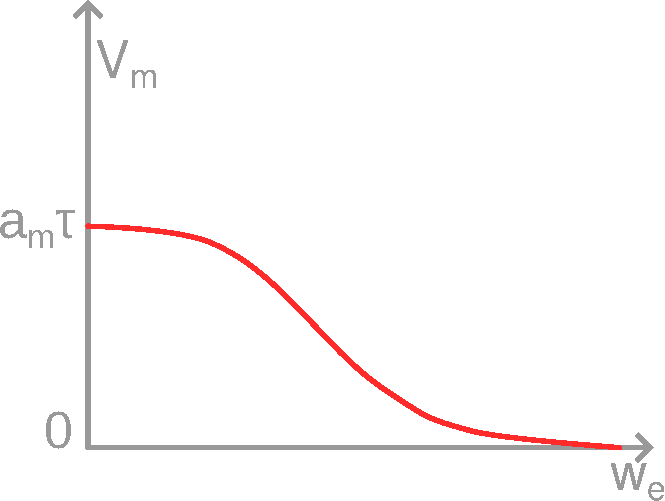
\includegraphics[scale=0.5]{s1}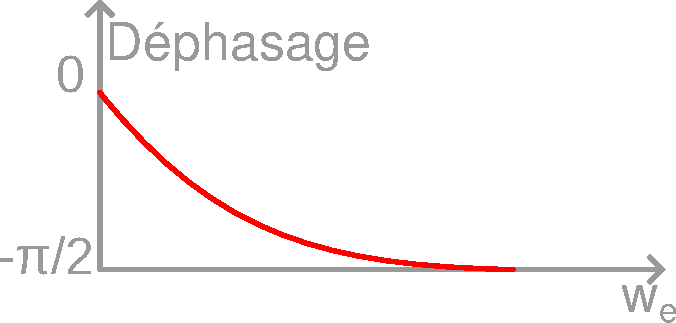
\includegraphics[scale=0.5]{s2}

Comme $\varphi_v(\omega_e) = \varphi_e - \arctan(\omega_e\tau)$, le déphasage tend vers $-\frac{\pi}{2}$.\marginInfo{La fonction arctan tend vers $\pi/2$ à l'infini.}
\section{Systèmes forcés du deuxième ordre}
\subsection{Exemple}
% Schéma 4
%
On fait varier la position de l'extrémité gauche du ressort $x_0$ de façon périodique au cours du temps. ${\color{red}x_0 = d_m \cos(\omega_e t+\varphi_e)}$ avec $d_m$ l'amplitude du mouvement et $\omega_e$ la fréquence.

PFD selon $\vec{e_x}$ : $m\ddot{x} = -k(x-x_0-l_0)$

On obtient $m\ddot{x} + kx = kl_0+k{\color{red}x_0(t)}$. En posant $X = x-l_0$ pour faire dispara\^itre $kl_0$, on a
\begin{flalign}
m\ddot{X} + kX &= k{\color{red}d_m\cos(\omega_e t+\varphi_e)}\notag\\
\ddot{X} + \frac{k}{m}X &= \frac{k}{m}d_m \cos(\omega_e t + \varphi_e)\notag\\
\ddot{X} + \omega_0^2X &= \omega_0^2 d_m \cos(\omega_e t + \varphi_e)\text{ avec } \omega_0 = \sqrt{\frac{k}{m}}\label{eq_4}
\end{flalign}
\subsection{Résolution sans dissipation}
On obtient une équation d'OH avec un second membre sinusoidal :
\begin{equation}
 \ddot{X} + \omega_0^2X = \omega_0^2 d_m \cos(\omega_e t + \varphi_e)\label{eq2}
\end{equation}
L'équation homogène associée est $\ddot{X} + \omega_0^2X = 0$, donc la solution homogène est $X_H(t) = A\cos(\omega_0 t) + B\sin(\omega_0 t)$.

On cherche une solution particulière $X_p(t)$ du m\^eme type que le second membre : sinusoidal avec la m\^eme pulsation $\omega_e$. Elle est de la forme $X_p(t) = X_m \cos(\omega_e t + \varphi_X)$ avec $X_m$ et $\varphi_x$ à déterminer.

\subsubsection{Introduction des grandeurs complexes}

$\underline{X_p} = X_me^{i(\omega_e t + \varphi_x)} = \underline{X_m} e^{i\omega_e t}$ avec $\underline{X_m} =  X_me^{i\varphi_x}$

$\underline{D} = d_m e^{i(\omega_e t + \varphi_e)} = \underline{d_m} e^{i\omega_e t} $ avec $\underline{d_m} = d_m e^{i\varphi_e}$

\subsubsection{Écriture de l'équation en complexe}
On réécrit \eqref{eq_4} avec les nouvelles grandeurs :
\begin{equation}
 \ddot{\underline{X_p}} + \omega_0^2 \underline{X_p} = \omega_0^2 \underline{D}\label{eq3}
\end{equation}
On a bien Re(\eqref{eq3}) = \eqref{eq2}.
\subsubsection{Calcul de la dérivée seconde et remplacement}
On calcule $\ddot{\underline{X_p}}$ :
$\dot{\underline{X_p}} = \underline{X_m} i\omega_e e^{i\omega_e t}$ et $\ddot{\underline{X_p}} = -\omega_e^2 \underline{X_m} e^{i\omega_e t}$\marginCritical{On trouve bien $i\omega_e^2$ car on rappelle que $i\times i = i^2 = -1$ !}.

On remplace dans \eqref{eq3} :

\begin{flalign}
-\omega_e^2 \underline{X_m} e^{i\omega_e t} + \omega_0 \times \underline{X_m}  e^{i\omega_e t} &= \omega_0^2 \underline{d_m} e^{i\omega_e t}\notag\\
\underline{X_m} (\omega_0^2 - \omega_e^2) &= \omega_0^2 \underline{d_m}\notag\\
\underline{X_m} &= \frac{\omega_0^2}{\omega_0^2 - \omega_e^2}\underline{d_m}
\end{flalign}
\subsubsection{Calcul des variables à determiner}
On calcule $X_m = |\underline{X_m}|$ et $\varphi_X = \arg(\underline{X_m})$.

$X_m = |\underline{X_m}| = |\frac{\omega_0^2}{\omega_0^2 - \omega_e^2}| \times |\underline{d_m}|$.

Si $\omega_0 > \omega_e, X_m = \frac{\omega_0^2}{\omega_0^2-\omega_e^2}d_m$ et si $\omega_0<\omega_e, X_m = \frac{\omega_0^2}{\omega_e^2-\omega_0^2}d_m$.
%\includegraphics{schema5}

$\varphi_X = \arg(\underline{X_m}) = \arg(\underline{d_m})+\arg(\omega_0^2)-\arg(\omega_0^2-\omega_e^2) = \varphi_e + 0 -\arg(\omega_0^2-\omega_e^2)$

Si $\omega_0 > \omega_e, \varphi_X = \varphi_e$\marginTips{En effet, l'argument d'un nombre négatif est $\pi$ et celui d'un positif est $0$}

Si $\omega_e > \omega_0, \varphi_X = \varphi_e-\pi$

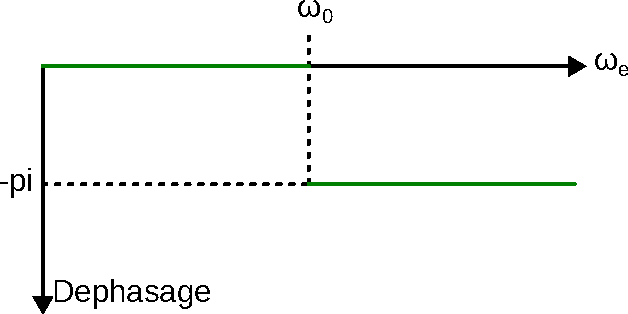
\includegraphics[scale=0.5]{deph_1}
\subsection{Résolution avec dissipation}
\subsubsection{Mise en équation}
On rajoute une force de frottement fluide $F = -\alpha \vec{v}$.

On fait le PFD selon $\vec{e_x} $: \begin{flalign}
m\ddot{x} &= -k(x-x_0-l_0) - \alpha \dot{x}\notag\\
m\ddot{x} + \alpha\dot{x} + k(x-l_0) = kx_0\notag\\
m\ddot{X}+\alpha\dot{X} + kX &= kx_0(t)\notag\\
\ddot{X}+\frac{\alpha}{m}\dot{X}+\frac{k}{m} X = \frac{k}{m} x_0(t)\notag\\
\ddot{X} + \frac{1}{\tau} \dot{X} + \omega_0^2X = \omega_0^2x_0(t)\label{eq_8}
\end{flalign}
En posant $\tau = \frac{m}{\alpha}$ et $\omega_0 = \sqrt{\frac{k}{m}}$ et en effectuant un changement de variable : $X = x-l_0$.
\subsubsection{Solution générale}
L'équation homogène associée à \eqref{eq_8} est :
\begin{equation}
\ddot{X_h} + \frac{1}{\tau}\dot{X_H} + \omega_0^2X_H  = 0\label{eq_h_2}
\end{equation}
Il s'agit d'une équation d'OH amorti dont la solution dépend du discriminant.\marginInfo{Voir le chapitre précédant pour la solution d'un OH amorti}
\subsubsection{Régime transitoire}
La solution de l’équation \eqref{eq_8} est la somme de la solution de l’équation sans second membre
et de la solution particulière. Compte tenu de la présence d’un amortissement, la solution
de l’équation sans second membre tend vers 0. au bout d’un temps suffisamment important,
seule la solution particulière reste non nulle. Seul le régime forcé
est étudié ici\marginInfo{Pour décrire le régime transitoire, il serait nécessaire
d’écrire la solution complète qui dépend des conditions initiales, mais ce n'est pas l'objet de cette partie.}. Pour le décrire, il suffit de rechercher la solution particulière.
\subsubsection{Mise en équation de la solution particulière}
On cherche maintenant une solution particulière $X_p(t)$

Elle doit vérifier
\begin{equation}
 \ddot{X_p} + \frac{1}{\tau}\dot{X_p} \omega_0^2X_p = \omega_0^2 d_m \cos(\omega_e t + \varphi_e)\label{eq_6}
\end{equation}



On cherche $X_p(t)$ sous la m\^me forme que le second membre, i.e \begin{equation}
                                                               X_P(t) = X_m\cos(\omega_et+\varphi_x)
                                                              \end{equation}
avec $\omega_e$ de m\^eme pulsation que l'excitation

\subsubsection{Introduction des grandeurs complexes}
$\underline{X_p} = X_me^{i(\omega_e t + \varphi_x)} = \underline{X_m} e^{i\omega_e t}$ avec $\underline{X_m} =  X_me^{i\varphi_x}$

$\underline{D} = d_m e^{i(\omega_e t + \varphi_e)} = \underline{d_m} e^{i\omega_e t} $ avec $\underline{d_m} = d_m e^{i\varphi_e}$

On réécrit \eqref{eq_6} avec les nouvelles grandeurs :
\begin{equation}
\ddot{\underline{X_p}} +  \frac{1}{\tau}\dot{\underline{X_p}} + \omega_0^2X_p = \underline{D}\label{eq_7}
\end{equation}

On calcule $\ddot{\underline{X_p}}$ :
$\dot{\underline{X_p}} = \underline{X_m} i\omega_e e^{i\omega_e t}$ et $\ddot{\underline{X_p}} = -\omega_e^2 \underline{X_m} e^{i\omega_e t}$.

On remplace dans \eqref{eq_7}\marginTips{En remplaçant les valeurs par leur écriture complexe, les exponentielles doivent se simplifier comme ici, si ce n'est pas le cas, c'est qu'il y a une erreur de calcul.} :

\begin{flalign}
-\omega_e^2 \underline{X_m} e^{i\omega_e t} +\frac{1}{\tau}\times \underline{X_m} i\omega_e e^{i\omega_e t} + \omega_0^2 \times \underline{X_m}  e^{i\omega_e t} &= \omega_0^2 \underline{d_m} e^{i\omega_e t}\notag\\
-\omega_e^2 \underline{X_m} \Ccancel[red]{e^{i\omega_e t}} +\frac{1}{\tau}\times \underline{X_m} i\omega_e \Ccancel[red]{e^{i\omega_e t}} + \omega_0^2 \times \underline{X_m}  \Ccancel[red]{e^{i\omega_e t}} &= \omega_0^2 \underline{d_m} \Ccancel[red]{e^{i\omega_e t}}\notag\\
\underline{X_m} (\omega_0^2 - \omega_e^2 + \frac{i\omega_e}{\tau}) &= \omega_0^2 \underline{d_m}\notag\\
\underline{X_m} = \frac{\omega_0^2}{\omega_0^2 - \omega_e^2 + \frac{i\omega_e}{\tau}}\underline{d_m}
\end{flalign}
On obtient $X_m = |\underline{X_m}|$ et $\varphi_x = \arg(\underline{X_m})$

On pose $u = \frac{\omega_e}{\omega_0}$. On a alors, en divisant par $\omega_0^2$.
\begin{flalign}
\underline{X_m} &= \frac{1}{1-\frac{\omega_e^2}{\omega_0^2} + \frac{\omega_e}{\omega_0} \frac{i\omega_e}{\tau}}\underline{d_m}\notag\\
&= \frac{1}{1-u^2 + \frac{iu}{Q}}\underline{d_m}\notag\\
&=  \frac{Q}{Q(1-u^2)+iu}\underline{d_m}
\end{flalign}

On calcule $X_m = |\underline{X_m}| = \frac{d_mQ}{\sqrt{Q^2(1-u^2)^2 + u^2}}$

Si $\omega_e\to 0$, le ressort se comporte comme une tige rigide et le déplacement de la masse vaut le déplacement de $x_0$

\subsubsection{Étude de la fonction}
On dérive la fonction :
\begin{flalign*}
d_mQ\times(-\frac{1}{2})\times \frac{Q^2\times 2 \times (1-u^2)\times(-2u) + 2u}{(Q^2(1-u^2)+u^2)^{3/2}}
\end{flalign*}
Elle vaut $0$ si $Q^2\times 2 \times (1-u^2)\times(-2u) + 2u = 0$, i.e. $u=0$ ou $u^2 = 1-\frac{1}{2Q^2}$. Si $Q\to\infty$, on tend vers le cas sans dissipation (OH).

Il existe une résonance seulement si $ 1-\frac{1}{2Q^2} >0 \iff Q > \frac{1}{\sqrt{2}}$.\marginInfo{ L'oscillateur est obligatoire en régime pseudo-périodique. Les condition de résonance sont uniquement sur $Q$ mais nécessite quand m\^eme un forçage.}
\includegraphics[scale=0.4]{Q}
\begin{itemize}
 \item Si $Q>\frac{1}{\sqrt{2}}$

Pulsation de la résonance : $u^2 = 1-\frac{1}{2Q^2} \iff \omega_e = \omega_0 \sqrt{1-\frac{1}{2Q^2}}$.

$X_m$ à la résonance : $X_m = \frac{d_mQ}{\sqrt{Q^2(1-u^2)^2 + u^2}} = \frac{d_mQ}{\sqrt{1-\frac{1}{4Q^2}}}$
\item Dans le cas contraire, la seule valeur de $u$ qui annule la dérivée est $u=0$, donc $u$ décroît, sans résonance.
\end{itemize}
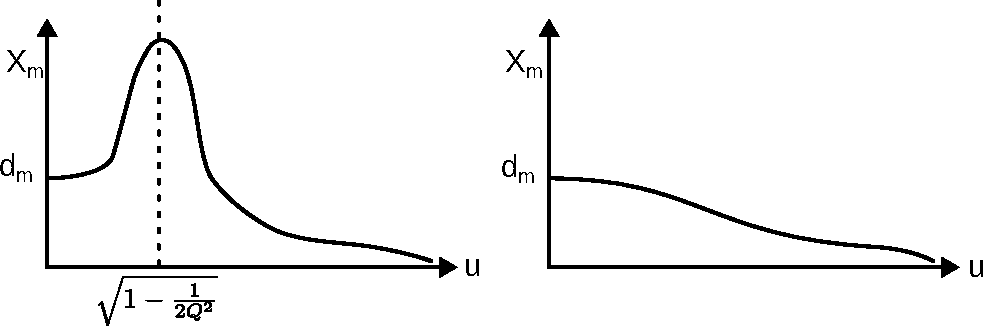
\includegraphics[scale=0.4]{resonance}

Si Q est très grand devant 1 qu'il tend vers l'infini par exemple, il y a une résonance pour $u = 1$ et l'amplitude maximale des oscillations de la masse est $d_m\times Q$.\marginInfo{En effet, si $Q>>1$, alors $\frac{d_mQ}{\sqrt{1-\frac{1}{4Q^2}}} \simeq \frac{d_mQ}{\sqrt{1}} = d_mQ$}

Si $Q=100, X_{m,max} = d_m\times 100$.
\subsubsection{Calcul de la phase}
$\varphi_X = \arg(\underline{X_m}) = \arg(\underline{d_m}) + \arg(Q)  - \arg(Q(1-u^2)+iu) = \varphi_e + 0 - \arg(Q(1-u^2)+iu)$.

Donc Si $u<1$, on a $\varphi_x = \varphi_e - \arctan(\frac{u}{Q(1-u^2)})$. Dans le cas contraire, on a $\varphi_x = \varphi_e - \arctan(\frac{u}{Q(1-u^2)}) - \pi$\marginTips{Si $a>0, \arg(a+ib) = \arctan(\frac{b}{a})$ ou $a>0, \arg(a+ib) = \arctan(\frac{b}{a})+\pi$}

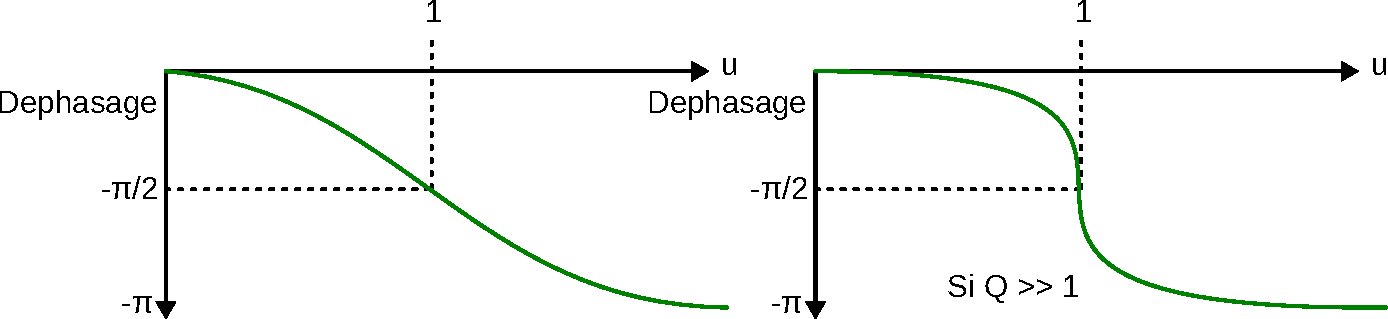
\includegraphics[scale=0.4]{deph-2}
\end{document}

